\section{Introduction}
\label{sec:introduction}

% Motivate the problem - why trust and emotion understanding is critical.

Two fatal self-driving-car accidents in March 2018 (Uber~\cite{uber} and Tesla~\cite{tesla}) have cast doubt in the general public on whether autonomous vehicles can become the future of personal transport. 
The Tesla accident happened in broad daylight in pretty much perfect driving conditions. Just days before that, an autonomous car prototype by Uber, equipped with LIDAR(s) completely vehicle failed to detect a pedestrian crossing the road at night. 
The autonomous vehicles industry, and research community, faces an uphill battle in convincing the public that self-driving cars are safer than human drivers.
As the framework for mobility in the United States begins to shift from one of personally-owned, manually-driven vehicles to one of a shared and partially automated fleet, established driver perceptions about their confidence, and trust in various vehicle technologies is now more than ever critical.
%to our understanding as to how one needs to facilitate behavior change.

Everyone is talking about autonomous vehicles. 
From automotive manufacturers, to consumer electronic giants, to software engineers, and academic researchers, self-driving cars are at the forefront of everyone’s imagination. 
There were more autonomous driving concepts at the International Consumer Electronics Show (CES) 2018 than ever before~\cite{techcrunch_2018}, demonstrating the seriousness, and commitment of many industries to bring autonomous cars to market.
Indeed AVs can make a meaningful difference to the world, enabling a new level of mobility, independence, and safety for all. 
This has been covered in reams of papers and many 1,000s of articles and news stories all over the globe. 
From questions of technological feasibility to thorny ethical dilemmas~\cite{lin2016ethics}, it’s been approached from many angles.
However there are aspects that haven’t yet been fully addressed - what do people want and need from AVs and how best to design for the user experiences - what about those human factors?
For example, we hypothesize that explaining why the vehicle is doing what it is doing to the passenger can increase their level of comfort in the autonomous vehicle.
The industry is preoccupied with the race to make their cars be as smart as possible and more safe than human drivers.
%What’s really important though, above all else, is how this technology can enable greater human mobility and hence improve their autonomy. 
Their approach to autonomy is imbalanced - there is too much focus on the discrete technologies that will enable it, with little regard for the powerful human factors involved. 
Naturally, one of the most important things to get right in AVs is safety. 
These vehicles must be incredibly safe, in fact safer, statistically and practically, than manually driven cars on the roads today if they’re to be of much use to us. 
%As the industry gets profoundly disrupted, we firmly believe that it’s not just automotive insiders who have a valuable contribution to make. 
According to a Deloitte study~\cite{deloitte}, trust and human behavior appears to be the biggest roadblock to adoption of self-driving cars in every country surveyed. 
%South Korea ranks the highest with $81\%$ of people expressing safety concerns about fully-autonomous vehicles. 
%China has the lowest figures, with $62\%$, but that still represents a large majority of consumers. 
The US falls roughly in the middle, where nearly three-quarters of consumers ($74\%$) believe that fully-autonomous vehicles will not be safe. 
%For the other countries in the study the percentage of consumers who believe fully-autonomous vehicle will not be safe are: Japan at $79\%$, Germany at $72\%$, and India at $64\%$
What is important is for car makers to rethink the design process to transform the entire user experience for the betterment, and safety of everyone. 
With that in mind - the goal of the proposed research is to utilize both human, and machine advantages to humanize autonomy by instilling the beneficial nuances of human behavior, emotion, and trust, while leveraging the technological and safety benefits of autonomous vehicles.
Beyond getting in and enjoying the ride – there are far more factors, details and nuances to be considered. 
What are the human factors at play here, and how can we design the best autonomous driving experience?

\begin{figure}
    \centering
    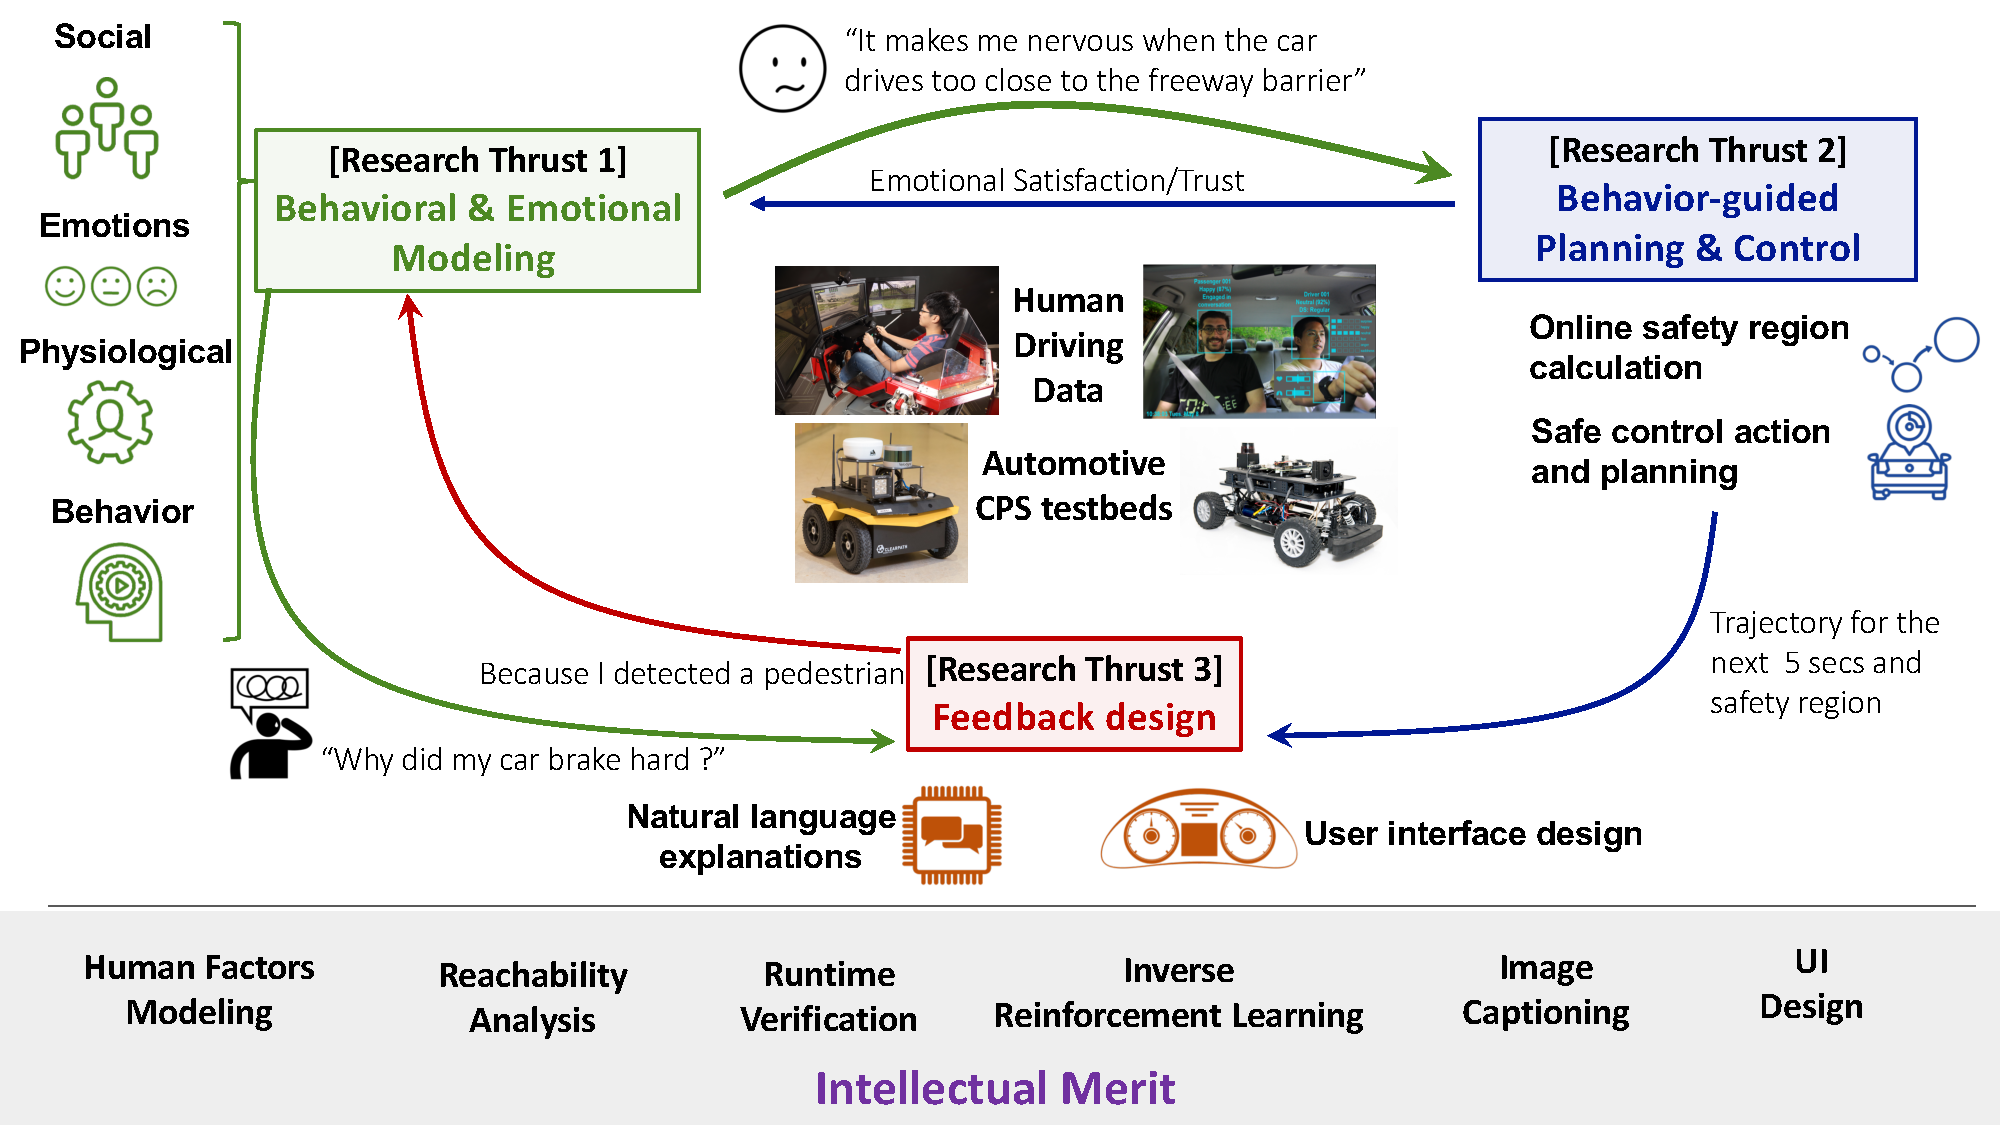
\includegraphics[width=0.8\columnwidth]{figures/overview_final.pdf}
    \caption{Overview of the three research trusts and their interconenctions}
    \label{fig:overview}
\end{figure}


%Despite the advances in technology, there is a fundamental fear and distrust of autonomous vehicles. 

While everyone wants AVs to be safe, the interpretation of safety, and the nature of trust in the vehicle or the system changes from person to person.
%Even for the same person, their perception of the trust in the autonomous vehicle varies based on their emotions and behavior.
Some perceive an autonomous vehicle in the same light as a malfunctioning robot, running amok around town, striking fear into passengers.
%On the other hand, even the sheer amazement experienced by those witnessing a fully autonomous car could cause a distraction and lead to accidents. 
Then there are those who believe and expect that the AV will always ``have your back'' and will be totally safe.
A quick YouTube search, reveals many videos where people are aware the systems have limitations, but still push them further than their intended use. %operating pilot assist systems on roads or situations when they shouldn't.
\textit{All of this boils down to one thing – human behavior}
Trust is one of the core human needs that the autonomous vehicle must establish and defend if the technology is to be adopted at all.
For the technology to be adopted, it must be trusted, and to do that, the human behavior and emotional needs must be taken into consideration. 


